\section{Track Trigger System Architecture\label{sec:tracktrigger}}


\subsection{CMS Outer Tracker Design and Simulation }


\subsection{System Architecture concept: divide and conquer in space and time }

	Processing each beam crossing implies finding and fitting thousands of tracks starting from a collection of Pt "stubs" (hit pairs, to be described earlier). We need to process 40 million beam crossing per second with a maximum latency of order of a few microseconds. The total raw computation power needed to solve this problem is huge, several orders of magnitude larger than what has ever been used for L1 triggering in the past. We obviously need to resort to massive parallelism and we choose to process in parallel different crossings coming at different times (time multiplexing) and different regions of the detector for the same crossing (regional multiplexing). For this purpose we divide the detector into 48 angular regions (n in $\eta$ times m in $\phi$) we call "towers". We assign multiple processing engines to each tower so that data from that  tower and from different crossings may be processed in parallel. In such a parallel system, a significant  problem we need to address and solve is how to dispatch the right data to the right processors. Data from the same crossing, coming from different detector elements, must be assembled and delivered to the same processing unit for track reconstruction. Data from different crossings, coming from the same detector element, must be delivered to different processing units for optimal time multiplexing. The subdivision of the detector into geographical towers, does not lead to an exact corresponding subdivision of the track parameter space. Data coming from a given geographical tower may need to be delivered to multiple parameter space regions. This happens, in particular, when a stub comes from a detector element close to the border between geographical towers, due to the finite curvature of charged particles in the magnetic field and finite size of the beam luminous region along the beam axis. In addition to the complex data dispatching challenge, there is the obvious challenge of finding and fitting many billions of tracks every second which requires extremely fast pattern recognition algorithms. 

 Current estimates show that only four microseconds will be available for track finding and fitting at L1. This includes data dispatching for trigger tower formation, pattern recognition, track fitting.  Data dispatching is where the stubs from many thousands silicon modules must be organized and delivered to the appropriate eta-phi trigger towers. Due to the finite size of the beam's luminous region in z and the finite curvature of charged particles in the magnetic field, some stubs must be duplicated and sent to multiple towers in an intelligent way. Since all this must be done within a very short time (of the order of a micro-second), communication between processing elements in different towers requires very high bandwidth and very low latency. In addition, extremely fast pattern recognition and effective track fitting is also required. Extensive $R\&D$ and experimentation of innovative ideas is obviously needed in these areas, and much of what have been done will be described in this paper.

	For the reasons above, the design of the overall architecture is focused on the need for efficient dispatching of the data for time and regional multiplexing and on the capability of providing a common flexible framework to test different possible solutions for track finding and fitting. Since the efficient data dispatching for time and regional multiplexing requires high bandwidth, low latency, and flexible real time communication among processing nodes, a full mesh communication based architecture is a natural fit. The full-mesh communication architecture can be implemented either with optical fibers or backplane. A custom ATCA board called Pulsar II, using the ATCA full-mesh backplane,  has been developed at Fermilab with the goal of creating a scalable architecture abundant in flexible, non-blocking, high bandwidth board-to-board communication channels. The Pulsar II hardware is the workhorse for the vertical slice demonstration. In addition, a pattern recognition mezzanine card is developed, as the pattern recognition engine. The full-mesh ATCA backplane permits high bandwidth inter-board communication. The full-mesh backplane is used to time-multiplex the high volume of incoming data in such a way that I/O demands are manageable at the board and chip level. The resulting architecture is scalable, flexible and enables us to provide an early technical demonstration using existing technology. The ATCA architecture allows us to explore and compare various pattern recognition architectures and algorithms within the same hardware platform. The detals of the Pulsar II hardware will be escribed later.
	
\noindent Track reconstruction typically consists of two steps: pattern recognition followed by track fitting. Pattern recognition involves choosing, among all the hits present in the detector, those hits that were potentially caused by the same particle. This stage produces a set of ”hits of interest”. Track fitting involves extracting track parameters from the coordinates of the ”hits of interest”. When time constraints are not so stringent, track reconstruction is implemented in software, often using processors running in the upper levels of a data acquisition system. However, software algorithms running on standard CPUs are typically not fast enough for low level triggers. 
 Hardware-based pattern recognition for fast silicon-based triggering on charged tracks was first developed for the CDF Silicon Vertex Trigger (SVT) at the Fermilab Tevatron in the 1990's.  The method used there~\cite{bib:Rist-89} was based on a massively parallel architecture - the Associative Memory - to efficiently identify patterns at high speed, and has provided an effective solution to fast track triggers in a hadron collider environment. It was successfully used in CDF in Run II at trigger Level 2 enabling a large number of physics results over more that 10 years. The same approach is now being implemented for ATLAS (FTK), also at Level 2, albeit with a much improved hardware architecture implemented with modern technology. However, applying associative memory approach to CMS Level 1 tracking trigger will require extensive $R\&D$ at all stages. 


	


\subsubsection{Tracker geometry and Trigger Towers }

\noindent Many unique challenges must be faced at the different stages of the processing chain: first, data need to be transferred out of the tracker at the necessary speed, stubs from thousands of silicon modules must be formatted, organized into $\eta - \phi$ trigger towers, duplicated and shared across tower boundaries as needed, then we need to perform pattern recognition and track fitting, and finally process all the tracks reconstructed by the previous stages to form an intelligent trigger decision. A coherent system design for a Level-1 track trigger will include all these aspects.

\noindent For the purpose of demonstration, we will make the working assumption that there will be a total of about 15K detector modules/fibers, each fiber with 5-10~Gbps payload bandwidth capability. The detector will be partitioned into 48 trigger towers, 6 in $\eta$ and 8 in $\phi$. Each trigger tower will therefore handle ~300 modules/fibers on average. The cabling of the modules will need to be optimized for trigger requirements. For simplicity, we will assume that the DAQ system are upstream and receive the fibers from the modules and pass the relevant data to the track trigger system. The focus here is the Vertical Slice Demonstration System, not the DAQ readout, so the DAQ readout details do not have to be involved in the demonstration.


\noindent The found stubs are sent from the modules using a block synchronous data transfer scheme which tolerates random occupancy fluctuations while bonding latency. The current plan is to have the data from 8 consecutive beam crossings as one block. The front-end designers are still investigating different format variants for robustness against rate fluctuations, ease of implementation, impact on power consumption, etc. While choosing the 8 crossings scheme as our current working assumption, our strategy is to design the downstream components to be flexible enough to handle different possible formats. 

\noindent Detailed studies have been done for the Barrel-Endcap (BE) tracker geometry with different trigger tower partitions, and the 6 (in $\eta$) x 8 (in $\phi$) = 48 trigger tower partition has been chosen as the default baseline configuration (see Figures~\ref{fig:SecDef_RZ}).

\begin{figure}[ht!]
\centering
\includegraphics[width=0.75\columnwidth]{Plots/SecDef_RZ.eps}
\includegraphics[width=0.2\columnwidth]{Plots/SecDef_XY.eps}
\caption{Six sectors in $\eta$ (left). Note that the symmetry around $\eta=0$ will provide for easier cable grouping. Eight sectors in phi (right).}
\label{fig:SecDef_RZ}
\end{figure}


\noindent Stubs from the 15K silicon modules must be delivered to the correct trigger towers. 
%Due to the finite size of the beam's luminous region in z and the finite $p_T$ curvature of charged particles in the magnetic field, some of %the stubs, coming from the neighborhood of some tower boundary, must be delivered to multiple towers to avoid efficiency gaps.  
Detailed studies have been performed on data sharing assuming the default 48 tower partition with a minimum $p_T$ of 2 GeV and track origin smearing in $z\pm 7$ cm. Figure~\ref{fig:TT_config} shows the number of trigger towers that stubs from a given module must be delivered to under these conditions. When a stub is in the middle of the trigger tower, it will have to be delivered to only one tower (to the native trigger tower). When a stub is at the boundary in phi or eta (but not both), it will have to be delivered to two towers. If a stub is at both the boundaries in eta and phi, it will have to be delivered to four towers. Note that four towers is the maximum number of towers any stub must be delivered to. 



\noindent The subdivision of the tracker into 48 trigger towers is shown in Figure~\ref{fig:TT_config} (right), where the colored lines indicate all needed interconnections among the trigger towers. The unique feature of this arrangement is that any given trigger tower only needs to be connected and share stubs with its immediate eight neighbors and detailed studies show that this feature is more or less independent from the minimum $p_T$ threshold and track origin smearing in $z$ requirements. This inter-connection structure will be used as the basis of the proposed trigger system architecture. 

\begin{figure}[ht!]
\centering
\includegraphics[width=0.45\columnwidth]{Plots/SecDef_N.eps}
\includegraphics[width=0.5\columnwidth]{Plots/CMS_L1_48_towers.png}
\caption{
Left: Distribution of the number of trigger towers each module needs to be connected to. Entries at zero are from modules that do not participate in triggering.
Right: Conceptual view of the proposed CMS phase II L1 tracking trigger towers.  The formation is organized as 48 trigger towers (6 $\eta$ x 8 $\phi$).  Because the phase II tracker is being designed for tracking trigger purposes, it is possible to arrange the towers in such a way that data sharing only requires communication with immediate neighbor towers.  Each node in this diagram represents a trigger tower processor engine.  Within each processor engine crate the full mesh backplane is used for time multiplexing of the incoming data, while the data sharing between towers is handled with inter-crate fiber links.}
\label{fig:TT_config}
\end{figure}



\subsubsection{System Architecture}

\noindent The tower processor platform must support large numbers of fiber transceivers, which are used for receiving input links and sharing data between neighboring towers.  A flexible, high bandwidth backplane is also required to quickly transfer data between boards.  The boards should be large enough to support pattern recognition engines and fiber connections. Given these requirements, we conclude that a full mesh 14 slot ATCA shelf is a natural fit for the tower processor. An ATCA shelf is typically an air-cooled 13U rack mounted chassis consisting of 14 slots.  The first two slots are reserved for Ethernet switch blades.  Switch blades may include a fast CPU and are often used for controls and other system functions.  The remaining 12 slots are used for processor or payload blades.  In a full mesh ATCA backplane each pair of slots is directly connected with a multi-lane bidirectional serial channel capable of supporting sustained 40+ Gbps data transfers.  A modern "40G+" full mesh ATCA shelf has a total aggregate bandwidth of over 7 Tbps, not including external I/O. As mentioned earlier, the full-mesh communication concept can be implemented either using full-mesh backplane, or using optical fibers. For  demonstration purpose, we will use the full-mesh backplane here. 

\noindent For simplicity and illustration purpose, let's simply assume one ATCA shelf per trigger tower for the moment as a starting point. This will be the assumption for the vertical slice demonstration. Following this assumption, if we were building the L1 Tracking Trigger system today using existing technology, we could propose a system comprised of 48 ATCA shevles with possibly an additional shelf acting as a second stage processor, as shown in Figs.~\ref{fig:System_1} and~\ref{fig:System_2} . Of course, the actual system will most likely be smaller (e.g. 24 or 12 shelves). Note that connections between tower processor shelves are limited to eight nearest neighbors, and this can be easily achieved.

\begin{figure}[ht!]
\centering
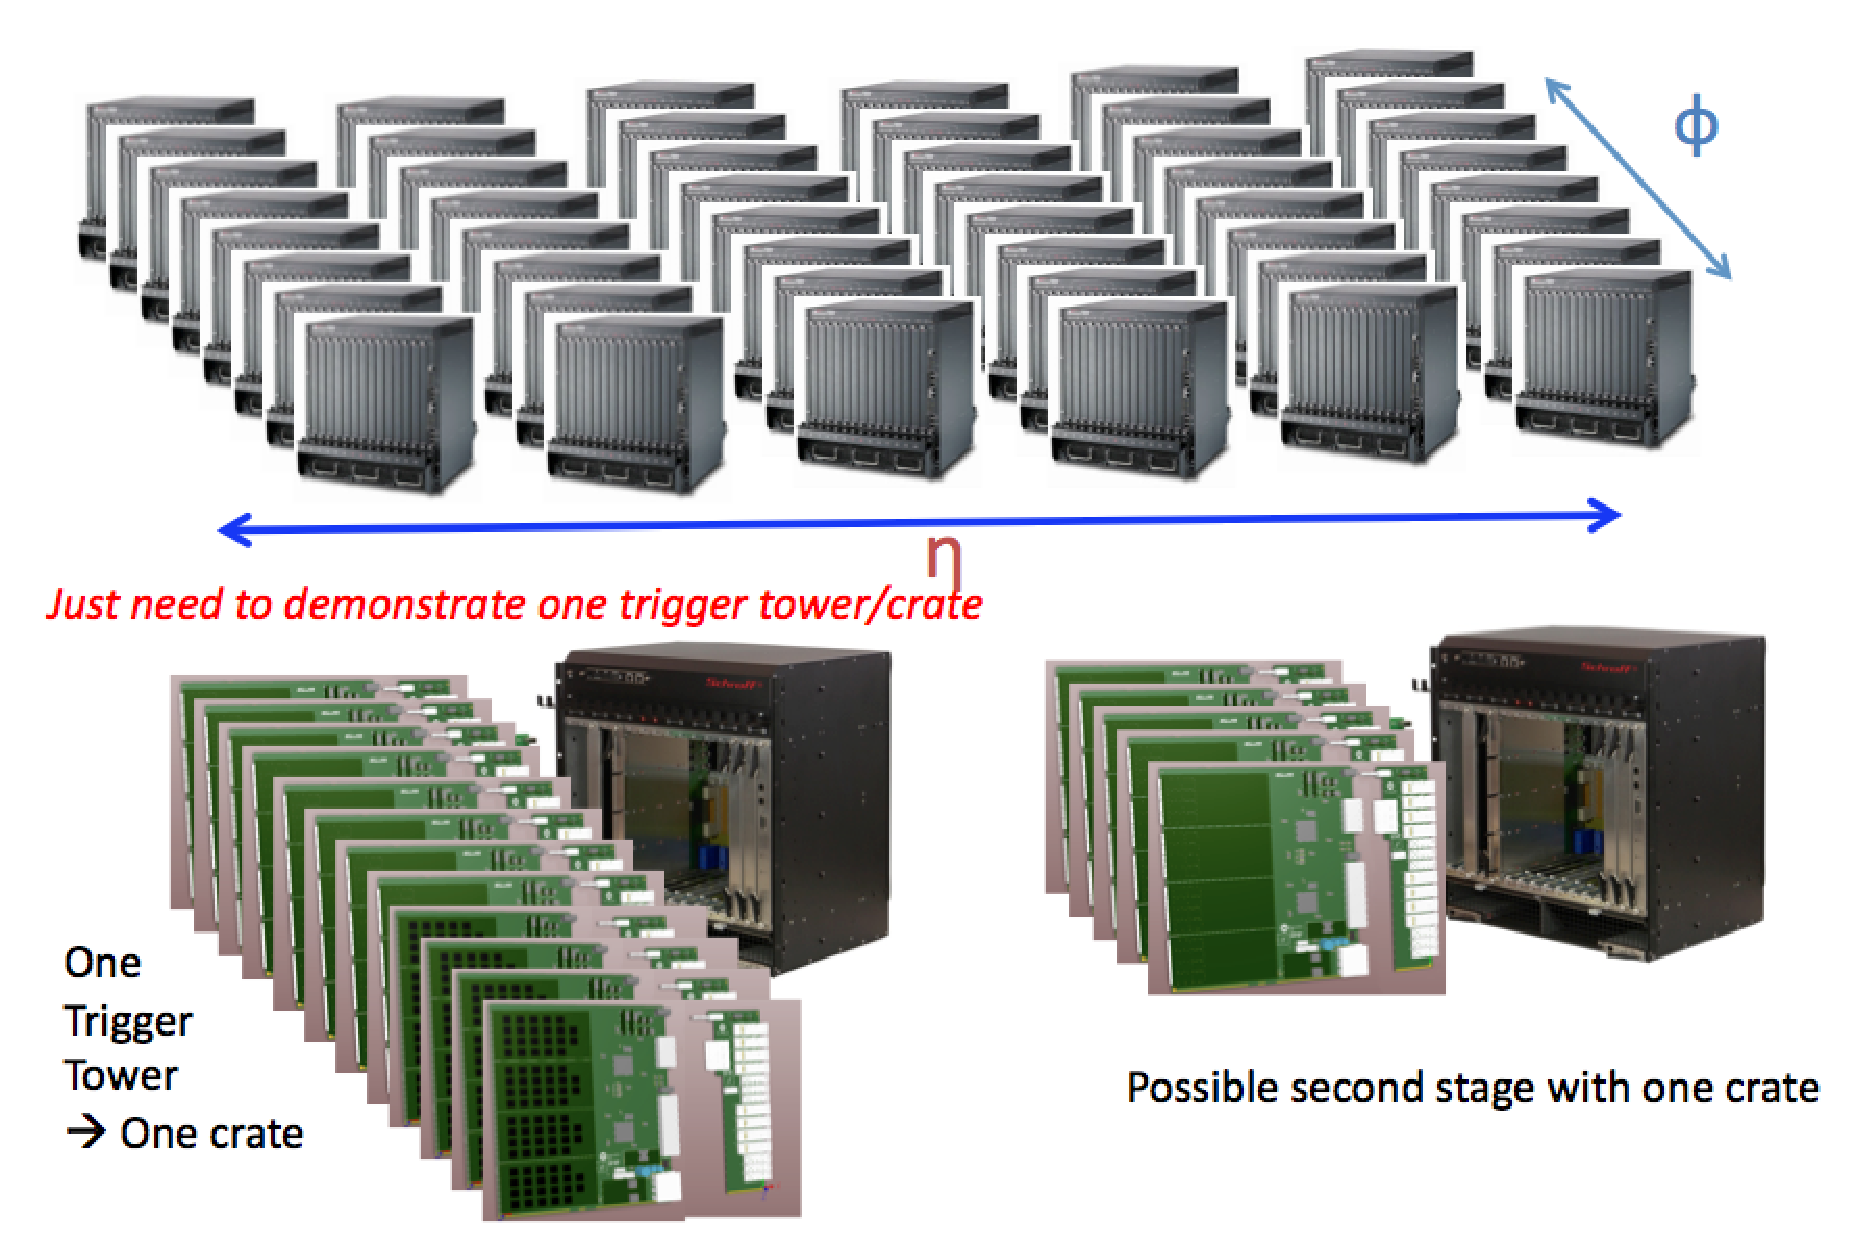
\includegraphics[width=0.7\columnwidth]{Plots/System_1.eps}
\caption{Possible system configuration with today's technology by simply assuming one ATCA shelf per trigger tower (will be smaller in the future for the actual system)}
\label{fig:System_1}
\end{figure}

\begin{figure}[ht!]
\centering
\includegraphics[width=0.5\columnwidth]{Plots/System_2.eps}
\caption{The second processing stage shelf.}
\label{fig:System_2}
\end{figure}



\begin{figure}[ht!]
\centering
\includegraphics[width=0.4\columnwidth]{Plots/ProcBlade.eps}
\includegraphics[width=0.4\columnwidth]{Plots/PulsarIIb.png}
\caption{Generic processor blade concept (left), and the actual design of Pulsar IIb~\cite{bib:PulsarII} at final layout stage (right)}
\label{fig:ProcBlade}
\end{figure}

\begin{figure}[ht!]
\centering
\includegraphics[width=0.4\columnwidth]{Plots/PRAM.eps}
\includegraphics[width=0.4\columnwidth]{Plots/test_mezzanine.png}
\caption{Left: Concept of a pattern recognition mezzanine design for testing different pattern recognition algorithms.
Right: a test mezzanine prototype designed and built at Fermilab, features four SFP+ pluggable serial transceivers (for standalone
data receiving), a Kintex 7 FPGA, configuration flash memory, DDR3 memory, power supplies, local oscillators, a test socket for
associative memory chips developed at Fermilab, and FMC connectors. 
}
\label{fig:PRAM}
\end{figure}

\noindent The generic processor blade concept is shown in Figure~\ref{fig:ProcBlade} (left).  The front board measures 8U x 280mm and is designed around a single FPGA.  This FPGA connects directly to the full mesh backplane fabric, mezzanine cards, and fiber transceivers located on a rear transition module (RTM).  For the most part communication channels are high speed serial point to point links and are directly supported by SERDES transceivers in the FPGA. The actual design of Pulsar IIb is also shown in Figure~\ref{fig:ProcBlade} (right).

\noindent The fundamental processing element is a pattern recognition mezzanine (PRM) card shown on Fig.~\ref{fig:PRAM} which performs both track finding and fitting. Time multiplexed data transfers into several parallel PRMs can reduce bandwidth requirement to manageable level.  PRM's using different approaches to track finding and fitting may be tested and compared within the same overall high-level system architecture and data dispatching scheme.


The system architecture described above is scalable, flexible and, although not meant to be what we
will actually implement in the final system, will enable us to provide an early technical demonstration
of the feasibility of a L1 tracking trigger for CMS. For example, a major advantage of the full mesh
communication (either via optical connection or via backplane) is that it effectively blurs the distinction between boards, thus enabling system architects to
experiment with different shelf configurations. In the following sections we briefly illustrate two kinds of
tower processor systems made possible by the flexibility of the full mesh architecture. (why this paragraph is repeating itself after compilation?....)


The system architecture described above is scalable, flexible.... testing testing.



\noindent

The system architecture described above is scalable, flexible and, although not meant to be what we will actually implement in the final system, will enable us to provide an early technical demonstration of the feasibility of a L1 tracking trigger for CMS. For example,
a major advantage of the full mesh backplane is that it effectively blurs the distinction between boards, thus enabling system architects to experiment with different shelf configurations.  In the following sections we briefly illustrate two kinds of tower processor systems made possible by the flexibility of the full mesh architecture.

\paragraph{N DIB and M PRM configuration ($N+M \le 12$)}

\noindent The most straightforward tower processor architecture consists of N data input boards (DIB), which receive input links and perform zero suppression.  After zero suppression, the N DIBs transfer the event data to M number of pattern recognition boards (PRB), which contain Mx4 pattern recognition mezzanine (PRM) cards.  Data transfers from the DIBs to the PRMs are time multiplexed, thereby the bandwidth requirements can be significantly relaxed.  

\noindent Data entering the PRB can be time multiplexed again and transferred to the four PRMs to further reduce bandwidth requirements and allow for longer processing times.  The full mesh backplane fabric supports any variant of these configurations (assuming that $N+M \le 12$), and different variants may have different demands on hardware. Example variations are sketched on Fig.\ref{fig:System_3} and bandwidth requirements for the worst case scenario (assuming 500 stubs per event per trigger tower) are summarized in Table~\ref{tab:shelves}. Note that current study show that on average, we expect only about 100 to 200 stubs per trigger tower per beam crossing, here we assumed 500 stubs to be conservative. 

\begin{figure}[ht!]
\centering
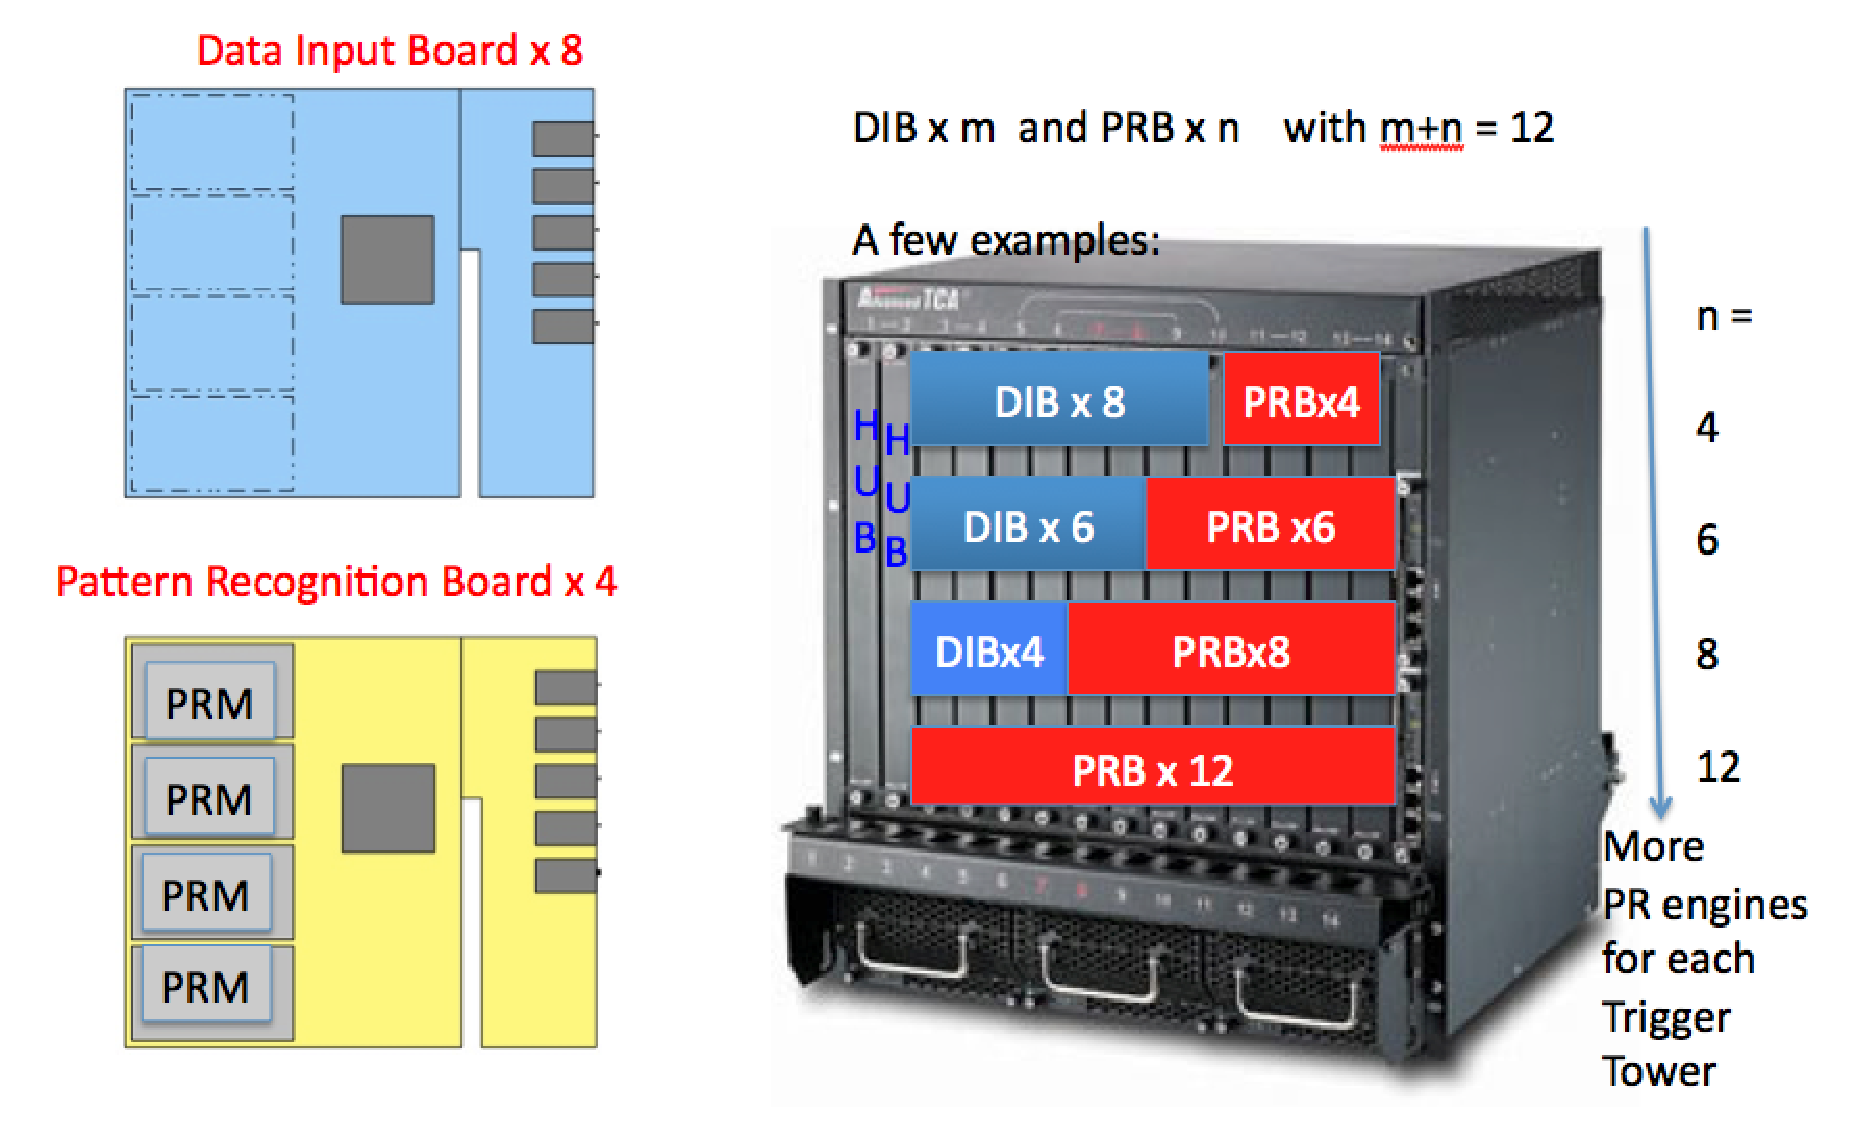
\includegraphics[width=0.7\columnwidth]{Plots/System_3.eps}
\caption{System flexibility: many configurations possible \& being studied to select the right one for demonstration purpose}
\label{fig:System_3}
\end{figure}


\begin{table}[ht!]
\centering\begin{tabular}{|c|c|c|c|c|}
\hline
DIB/PRB/PRM Count &  Fabric Channel BW (minimum)  &	PRM Input BW (minimum) \\
8/4/16 &	20 Gbps &	40 Gbps \\
6/6/24 &	20 Gbps &	27 Gbps \\
4/8/32 &	20 Gbps &	20 Gbps \\
\hline
\end{tabular}
\caption{Data sharing between towers occurs on the PRB board level.  Each PRB connects to the corresponding PRB in the eight nearest tower processor shelves.  The above numbers assume a worst case scenario of 500 32-bit stubs per trigger tower per event (every 25 ns).  An example of special configuration with eight DIBs and four PRBs will be used as a simple example in Section 3.}
\label{tab:shelves}
\end{table}


\paragraph{DIB/PRB combo configuration}

\noindent In the limit of N=0 and M=12 from the "N DIB and M PRB" configuration, the DIB and PRB functionalities can be combined into one blade design.

%\begin{figure}[ht!]
%\centering
%\includegraphics[width=0.45\columnwidth]{Plots/CombBlade.eps}
%\caption{Combined blade design}
%\label{fig:CombBlade}
%\end{figure}


\noindent A tower shelf would then consist of 10 Processor blades, one Gateway blade (for data sharing), and one Collector blade (for tracks found). These three different blade functionalities can be implemented in the same hardware. Backplane transfers are described in a series of fully pipelined sequences shown in Figure~\ref{fig:BackPlaneTr}.

\begin{figure}[ht!]
\centering
\includegraphics[width=0.9\columnwidth]{Plots/BackPlaneTr.eps}
\caption{Backplane transfers sequences using the combined blade design. First, the input fibers are received on the Processor blades (a).  Each Processor blade then transfers a portion of the input data to the Gateway blade (b), where it is exchanged with neighboring towers over fiber links (c).  The Processor blades and Gateway blade transfer the event (including neighbor data) to the target Processor blade in a time multiplexed, round robin scheme (d).   Results from the Processor blades are then transferred to the Collector blade (e) for any final formatting and processing before transmission downstream (f).}
\label{fig:BackPlaneTr}
\end{figure}
 

\noindent This processor architecture uses every channel in the full mesh backplane.  By using the full mesh fabric more effectively we are able to decrease the channel bandwidth requirement from 20 Gbps down to 6 Gbps with no significant latency increase. 



\subsection{Applying Associative Memory approach to CMS }



\subsubsection{Pattern Bank definition and optimization through simulation }


\subsubsection{Comparison between SVT, FTK and CMS L1 tracking trigger }






%\clearpage

